\section{The Orienteering Problem}

\begin{frame}{The Orienteering Problem}

	\note<1>[item]{
		Proper definition of the OP \begin{itemize}
			\item Start with an undirected graph
			\item Cost function $t$ for the edges \begin{itemize}
				      \item Also \enquote{distance}, \enquote{travel time}, \enquote{weight}
			      \end{itemize}
			\item Profit function $s$ for the nodes \begin{itemize}
				      \item Also \enquote{score}
			      \end{itemize}
			\item Maximum cost $T_{max}$
		\end{itemize}
	}
	\note<2>[item]{
		Orienteering Problem \begin{itemize}
			\item Want a path from $v_1$ to $v_n$ \begin{itemize}
				      \item Need not be fixed but often are
				      \item Named like this for convenience
			      \end{itemize}
			\item Path should maximize the total profit...
			\item ...while respecting the cost limit $T_{max}$
		\end{itemize}
	}
	\note<2>[item]{Questions?}

	\begin{definition}[Orienteering Problem \cite{vansteenwegen_orienteering_2011}]
		Let $G=(V = \{v_1, \dots, v_n\}, E)$ be an undirected graph with a cost function $t: E \rightarrow \mathbb{R}_+$
		and a profit function $s: V \rightarrow \mathbb{R}$.
		Also, let $T_{max} \in \mathbb{R}_+$ be a cost limit.

		\only<2->{
		The \oplong{} aims at finding a path $P = [p_1, \dots, p_k], p_i \in V$ with $p_1 = v_1$ and ending at $p_k = v_n$
		which maximizes the total profit $S(P) := \sum_{p_i \in P} s(p_i)$ while respecting the cost limit, that is
		\begin{equation*}
			T(P) := \sum_{i = 1}^{k-1} t(v_i, v_{i+1}) \leq T_{max}
		\end{equation*}
		}
	\end{definition}

\end{frame}

\begin{frame}{Example}

	\note<1>[item]{
		Example OP instance \begin{itemize}
			\item $T_{max} = 6$
			\item Edges between all nodes (omitted for clarity)
			\item Horizontal/Vertical distance between neighboring nodes: 1
			\item Diagonal movement: $\sqrt 2 \approx 1.4$
		\end{itemize}}
	\note<1>[item]{Ask audience: What is the optimal path?}
	\note<2>[item]{Best path as far as I can see}

	\centering
	\begin{columns}
		\begin{column}{0.48\textwidth}
			\begin{itemize}
				\item<1-> Grid spacing of $1$
				\item<1-> $T_{max} = 6$
				\item<2> $T(P) = 4 + \sqrt 2 < 6$
				\item<2> $S(P) = 28$
			\end{itemize}
		\end{column}
		\begin{column}{0.48\textwidth}
			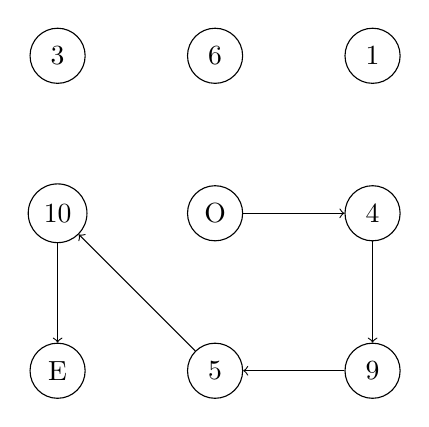
\begin{tikzpicture}[every node/.style={draw,shape=circle,minimum size=7mm}]
				\node (origin) at (0,0) {O};
				\node (1) at (-2,0) {10};
				\node (2) at (-2,2) {3};
				\node (3) at (0,2) {6};
				\node (4) at (2,0) {4};
				\node (5) at (0,-2) {5};
				\node (6) at (2,-2) {9};
				\node (7) at (2,2) {1};
				\node (end) at (-2,-2) {E};

				\draw<2>[->] (origin) -- (4);
				\draw<2>[->] (4) -- (6);
				\draw<2>[->] (6) -- (5);
				\draw<2>[->] (5) -- (1);
				\draw<2>[->] (1) -- (end);
			\end{tikzpicture}
		\end{column}
	\end{columns}
\end{frame}

\begin{frame}{Complete Graphs}

	\note<1>[item]{
		Getting into the problem \begin{itemize}
			\item Restrictions on allowed input graphs
			\item Introduce common ones in order of strictness
			\item After: introduce algorithms and try to reduce the restrictions they require
		\end{itemize}
	}
	\note<2->[item]{First: Complete Graph}
	\note<2->[item]{
		Probably known to everyone \begin{itemize}
			\item But for completeness' sake
		\end{itemize}
	}
	\note<3->[item]{
		Almost unanimous
	}
	\note<4->[item]{
		Simple to transform any graph into complete graph. Insert missing edges with weight \begin{itemize}
			\item Weight of the shortest path between nodes
			\item $\infty$ if the missing edges should not be taken \begin{itemize}
				      \item Might not work for all algorithms though (example later)
			      \end{itemize}
		\end{itemize}
	}

	\only<2->{
		\begin{definition}[Complete Graphs]
			A graph $G = (V, E)$ is \emph{complete} if for any two nodes $v_i \neq v_j \in V$ there exists a corresponding edge $\{v_i, v_j\} \in E$.
		\end{definition}
	}

	\begin{itemize}
		\item<3-> Almost unanimous in the literature \cite{vansteenwegen_orienteering_2011,laporte_selective_1990,santini_hazardous_2022,szwarc_novel_2022}
		\item<4-> Simple to transform any graph into a complete graph \begin{itemize}
			\item Might be computationally expensive on large inputs
		\end{itemize}
	\end{itemize}
\end{frame}

\begin{frame}{Triangle Inequality}
	\note<1->[item]{
		First actual restriction \begin{itemize}
			\item Similarly defined as in geometry
		\end{itemize}
	}
	\note<2->[item]{
		Any three nodes' weights satisfy the triangle inequality
	}
	\note<3->[item]{
		$\Rightarrow$ The direct edge is always the shortest path between nodes. \begin{itemize}
			\item No detour will ever be faster
		\end{itemize}
	}
	\note<4->[item]{Less often explicitly stated in literature}
	\note<4->[item]{
		Usually implied as part of Euclidean Metric \begin{itemize}
			\item Defined shortly
		\end{itemize}
	}

	\only<2->{
		\begin{definition}[Triangle Inequality \cite{black_triangle_2004}]
			A complete, weighted graph $G = (V, E)$ satisfies the \emph{triangle inequation}
			if any three nodes $u \neq v \neq w \in V$ statisfy the following inequality:
			\begin{displaymath}
				t(u,w) \leq t(u,v) + t(u,v)
			\end{displaymath}
		\end{definition}
	}

	\begin{itemize}
		\item<3->[$\Rightarrow$] The direct edge is always the shortest path between nodes.
		\item<4-> Less often explicitly stated \cite{santini_hazardous_2022}
		\item<4-> More often implied by requiring a Euclidean metric
	\end{itemize}
\end{frame}

\begin{frame}{Triangle Inequality}

	\note<1>[item]{What do we get out of this?}
	\note<2>[item]{Many problems: better approximations on more restricted graphs}
	\note<2>[item]{
		Easier to reason about rest of graph \begin{itemize}
			\item example following now
		\end{itemize}
	}
	\note<3->[item]{Simple greedy algorithm}
	\note<4->[item]{
		We always want to pick a node per step \begin{itemize}
			\item Navigating to that node and then to the end may not violate $T_{max}$
			\item Maximize the ratio between score gained and distance traveled
		\end{itemize}
	}
	\note<4->[item]{
		If no such node, go to the end
	}

	\begin{itemize}
		\item<2> Many problems have better approximations on such graphs \cite{black_triangle_2004}
		\item<2> Easier to reason about the rest of the graph.
		\item<3-> Simple greedy algorithm \begin{itemize}
			\item<4-> Let $P = [p_1, \dots, p_k]$ is the current path
			\item<4-> Always pick the node $v \in V \setminus P$ such that
			\begin{equation*}
				T(P \cup [v, v_n]) \leq T_{max}
			\end{equation*}
			and
			\begin{equation*}
				\frac{s(v)}{t(p_k, v)}
			\end{equation*}
			is maximized.
		\end{itemize}
		\item<4-> If no such node exists, go to the end node.
	\end{itemize}
\end{frame}

\begin{frame}{Example}

	\note<4->{
		Z.B. jetzt \begin{itemize}
			\item Remaining capacity of around $2.35$.
			\item To which node can we go (and then to the end) without volating $T_{max}$?
			\item[$\Rightarrow$] Only the node $5$
		\end{itemize}
	}
	\note<4->{
		Technically we could travel to node $4$ instead without immediately violating $T_{max}$ \begin{itemize}
			\item But travelling to the end then would violate it.
			\item Since we know this: Triangle Inequality $\Rightarrow$ There is no shorter way
			\item[$\Rightarrow$] Travelling to $4$ does not allow reaching the end
		\end{itemize}
	}
	\note<4->{
		Both algorithms presented today, rely on this fact
	}

	\centering
	\begin{tikzpicture}[every node/.style={draw,shape=circle,minimum size=7mm}]
		\node (origin) at (0,0) {O};
		\node<1> (1) at (-2,0) {10};
		\node<2-> (1) at (-2,0) {10};
		\node (2) at (-2,2) {3};
		\node (3) at (0,2) {6};
		\node (4) at (2,0) {4};
		\node (5) at (0,-2) {5};
		\node (6) at (2,-2) {9};
		\node (7) at (2,2) {1};
		\node (end) at (-2,-2) {E};

		\node[draw=none,right=2cm of 7] (b) {$T_{max} = 7$};
		\node<1>[draw=none,right=2cm of 4] (a) {$T(P) = 0$};
		\node<2>[draw=none,right=2cm of 4] (a) {$T(P) = 1$};
		\node<3>[draw=none,right=2cm of 4] (a) {$T(P) \approx 2.41$};
		\node<4>[draw=none,right=2cm of 4] (a) {$T(P) \approx 4.65$};
		\node<5>[draw=none,right=2cm of 4] (a) {$T(P) \approx 5.65$};
		\node<6>[draw=none,right=2cm of 4] (a) {$T(P) \approx 6.65$};

		\draw<2->[->] (origin) -- node[draw=none,above] {$1$} (1);
		\draw<3->[->] (1) -- node[draw=none,above left] {$\sqrt 2$} (3);
		\draw<4->[->] (3) -- node[draw=none,above right] {$\sqrt 5$} (6);
		\draw<5->[->] (6) -- node[draw=none,above] {$1$} (5);
		\draw<6->[->] (5) -- node[draw=none,above] {$1$} (end);
	\end{tikzpicture}
\end{frame}

\begin{frame}{Euclidean Metric}
	\note<1->{Definition like in geometry}
	\note<1->{
		Nodes are points in the euclidean plane \begin{itemize}
			\item Edge weights are distances between them
		\end{itemize}
	}
	\note<2->{
		Note, that this entails completeness and the triangle inequality \begin{itemize}
			\item[$\Rightarrow$] Entails the previous two restrictions
		\end{itemize}
	}
	\note<2->{Commonly seen in the literature}

	\begin{definition}
		For every node $v_i \in V$, there are coordinates $(x_i,y_i)^\intercal \in \mathbb{R}^2$
		and for each pair of nodes $v_i \neq v_j \in V$ the edge weights are defined as:
		\begin{displaymath}
			t(v_i,v_j) := \sqrt{(x_i - x_j)^2 + (y_i - y_j)^2}
		\end{displaymath}
	\end{definition}

	\begin{itemize}
		\item<2-> Entails the previous two restrictions
    \item<2-> Very common in the literature \cite{geem_harmony_2005,golden_orienteering_1987,szwarc_novel_2022,tsiligiridis_heuristic_1984}
	\end{itemize}
\end{frame}
